\qrchapterstar{https://forgottenpillar.com/rsc/en-fp-appendix}{Appendix} \label{chap:appendix}


\qrchapterstar{https://forgottenpillar.com/rsc/en-fp-appendix}{ملحق} \label{chap:appendix}


\addcontentsline{toc}{chapter}{Appendix}


\addcontentsline{toc}{chapter}{ملحق}


\section*{The Fundamental Principles 1889}


\section*{المبادئ الأساسية 1889}


As elsewhere stated, Seventh-day Adventists have no creed but the Bible; but they hold to certain well-defined points of faith for which they feel prepared to give a reason “to every man that asketh” them. The following propositions may be taken as a summary of the principal features of their religious faith, upon which there is, so far as we know, entire unanimity throughout the body. They believe,—


كما ذُكر في مواضع أخرى، ليس للأدفنتست السبتيين عقيدة سوى الكتاب المقدس؛ لكنهم يتمسكون بنقاط محددة جيدًا من الإيمان يشعرون أنهم مستعدون لتقديم سبب “لكل من يسألهم”. يمكن اعتبار المقترحات التالية ملخصًا للسمات الرئيسية لإيمانهم الديني، والتي يوجد، على حد علمنا، إجماع تام عليها في جميع أنحاء الجماعة. هم يؤمنون،-


\lettrine{I.} That there is one God, a personal, spiritual being, the creator of all things, omnipotent, omniscient, and eternal; infinite in wisdom, holiness, justice, goodness, truth, and mercy; unchangeable, and everywhere present by his representative, the Holy Spirit. Psalm 139:7.


\lettrine{I.} أن هناك إله واحد، كائن شخصي روحي، خالق كل الأشياء، قدير وعليم وأبدي؛ لا نهائي في الحكمة والقداسة والعدل والصلاح والحق والرحمة؛ لا يتغير، وموجود في كل مكان بواسطة ممثله، الروح القدس. مزمور 139:7.


\lettrine{II.} That there is one Lord Jesus Christ, the Son of the Eternal Father, the one by whom he created all things, and by whom they do consist; that he took on him the nature of the seed of Abraham for the redemption of our fallen race; that he dwelt among men, full of grace and truth, lived our example, died our sacrifice, was raised for our justification, ascended on high to be our only mediator in the sanctuary in heaven, where, through the merits of his shed blood, he secures the pardon and forgiveness of the sins of all those who penitently come to him; and as the closing portion of his work as priest, before he takes his throne as king, he will make the great atonement for the sins of all such, and their sins will then be blotted out (Acts 3:19) and borne away from the sanctuary, as shown in the service of the Levitical priesthood, which foreshadowed and prefigured the ministry of our Lord in heaven. See Leviticus 16; Hebrews 8:4, 5; 9:6, 7; etc.


\lettrine{II.} أن هناك رب واحد يسوع المسيح، ابن الآب الأبدي، الذي به خلق كل الأشياء، وبه تقوم؛ وأنه أخذ على نفسه طبيعة نسل إبراهيم لفداء جنسنا الساقط؛ وأنه سكن بين الناس، مملوءًا نعمة وحقًا، وعاش قدوتنا، ومات ذبيحتنا، وأُقيم لتبريرنا، وصعد إلى العلى ليكون وسيطنا الوحيد في القدس في السماء، حيث، من خلال استحقاقات دمه المسفوك، يؤمن الغفران والصفح عن خطايا جميع الذين يأتون إليه تائبين؛ وكجزء ختامي من عمله ككاهن، قبل أن يأخذ عرشه كملك، سيقدم الكفارة العظيمة عن خطايا كل هؤلاء، وستُمحى خطاياهم حينئذ (أعمال 3:19) وتُحمل بعيدًا عن المقدس، كما هو موضح في خدمة الكهنوت اللاوي، الذي سبق وصوّر خدمة ربنا في السماء. انظر لاويين 16؛ عبرانيين 8:4، 5؛ 9:6، 7؛ إلخ.


\lettrine{III.} That the Holy Scriptures of the Old and New Testaments were given by inspiration of God, contain a full revelation of his will to man, and are the only infallible rule of faith and practice.


\lettrine{III.} أن الكتب المقدسة للعهدين القديم والجديد أُعطيت بوحي من الله، وتحتوي على إعلان كامل لإرادته للإنسان، وهي القاعدة الوحيدة المعصومة للإيمان والممارسة.


\lettrine{IV.} That baptism is an ordinance of the Christian church, to follow faith and repentance,—an ordinance by which we commemorate the resurrection of Christ, as by this act we show our faith in his burial and resurrection, and through that, in the resurrection of all the saints at the last day; and that no other mode more fitly represents these facts than that which the Scriptures prescribe, namely, immersion. Romans 6:3-5; Colossians 2:12.


\lettrine{IV.} أن المعمودية هي فريضة من فرائض الكنيسة المسيحية، تتبع الإيمان والتوبة - فريضة نحتفل بها بقيامة المسيح، لأننا بهذا العمل نُظهر إيماننا بدفنه وقيامته، ومن خلال ذلك، بقيامة جميع القديسين في اليوم الأخير؛ وأنه لا توجد طريقة أخرى تمثل هذه الحقائق بشكل أفضل من تلك التي يصفها الكتاب المقدس، وهي التغطيس. رومية 6:3-5؛ كولوسي 2:12.


\lettrine{V.} That the new birth comprises the entire change necessary to fit us for the kingdom of God, and consists of two parts; First, a moral change wrought by conversion and a Christian life (John 3:3, 5); second, a physical change at the second coming of Christ, whereby, if dead, we are raised incorruptible, and if living, are changed to immortality in a moment, in the twinkling of an eye. Luke 20:36; 1 Corinthians 15:51, 52.


\lettrine{V.} أن الولادة الجديدة تشمل التغيير الكامل اللازم لتأهيلنا لملكوت الله، وتتكون من جزأين؛ أولاً، تغيير أخلاقي يحدث بالتحول وحياة مسيحية (يوحنا 3:3، 5)؛ ثانيًا، تغيير جسدي عند المجيء الثاني للمسيح، حيث، إن كنا أمواتًا، نُقام غير فاسدين، وإن كنا أحياء، نتغير إلى عدم الموت في لحظة، في طرفة عين. لوقا 20:36؛ 1 كورنثوس 15:51، 52.


\lettrine{VI.} That prophecy is a part of God’s revelation to man; that it is included in that Scripture which is profitable for instruction (2 Timothy 3:16); that it is designed for us and our children (Deuteronomy 29:29); that so far from being enshrouded in impenetrable mystery, it is that which especially constitutes the word of God a lamp to our feet and a light to our path (Psalm 119:105; 2 Peter 1:19); that a blessing is pronounced upon those who study it (Revelation 1:1-3); and that, consequently, it is to be understood by the people of God sufficiently to show them their position in the world’s history and the special duties required at their hands.


\lettrine{VI.} أن النبوة هي جزء من إعلان الله للإنسان؛ وأنها مشمولة في ذلك الكتاب المقدس الذي هو نافع للتعليم (2 تيموثاوس 3:16)؛ وأنها مصممة لنا ولأولادنا (تثنية 29:29)؛ وأنها بعيدة كل البعد عن أن تكون مغلفة بغموض لا يمكن اختراقه، بل هي التي تشكل بشكل خاص كلمة الله سراجًا لأقدامنا ونورًا لسبيلنا (مزمور 119:105؛ 2 بطرس 1:19)؛ وأن بركة تُعلن على أولئك الذين يدرسونها (رؤيا 1:1-3)؛ وبالتالي، يجب أن يفهمها شعب الله بما يكفي لإظهار موقفهم في تاريخ العالم والواجبات الخاصة المطلوبة منهم.


\lettrine{VII.} That the world’s history from specified dates in the past, the rise and fall of empires, and the chronological succession of events down to the setting up of God’s everlasting kingdom, are outlined in numerous great chains of prophecy; and that these prophecies are now all fulfilled except the closing scenes.


\lettrine{VII.} أن تاريخ العالم من تواريخ محددة في الماضي، وصعود وسقوط الإمبراطوريات، والتسلسل الزمني للأحداث وصولاً إلى إقامة ملكوت الله الأبدي، مخطط في سلاسل عديدة عظيمة من النبوءات؛ وأن هذه النبوءات كلها قد تحققت الآن باستثناء المشاهد الختامية.


\lettrine{VIII.} That the doctrine of the world’s conversion and a temporal millennium is a fable of these last days, calculated to lull men into a state of carnal security, and cause them to be overtaken by the great day of the Lord as by a thief in the night (1 Thessalonians 5:3); that the second coming of Christ is to precede, not follow, the millennium; for until the Lord appears, the papal power, with all its abominations, is to continue (2 Thessalonians 2:8), the wheat and tares grow together (Matthew 13:29, 30, 39), and evil men and seducers wax worse and worse, as the word of God declares. 2 Timothy 3:1, 13.


\lettrine{VIII.} أن عقيدة تحول العالم وألفية زمنية هي خرافة من هذه الأيام الأخيرة، مصممة لتهدئة الناس في حالة من الأمان الجسدي، وتجعلهم يفاجأون بيوم الرب العظيم كلص في الليل (1 تسالونيكي 5:3)؛ وأن المجيء الثاني للمسيح سيسبق الألفية، وليس يتبعها؛ لأنه حتى يظهر الرب، ستستمر القوة البابوية، بكل رجاساتها (2 تسالونيكي 2:8)، وينمو القمح والزوان معًا (متى 13:29، 30، 39)، ويزداد الأشرار والمضلون شرًا، كما تعلن كلمة الله. 2 تيموثاوس 3:1، 13.


\lettrine{IX.} That the mistake of Adventists in 1844 pertained to the nature of the event then to transpire, not to the time; that no prophetic period is given to reach to the second advent, but that the longest one, the two thousand and three hundred days of Daniel 8:14, terminated in 1844, and brought us to an event called the cleansing of the sanctuary.


\lettrine{IX.} أن خطأ الأدفنتست في عام 1844 كان يتعلق بطبيعة الحدث الذي كان سيحدث آنذاك، وليس بالوقت؛ وأنه لا توجد فترة نبوية معطاة تصل إلى المجيء الثاني، ولكن أطولها، الألفين وثلاثمائة يوم من دانيال 8:14، انتهت في عام 1844، وأوصلتنا إلى حدث يسمى تطهير المقدس.


\lettrine{X.} That the sanctuary of the new covenant is the tabernacle of God in heaven, of which Paul speaks in Hebrews 8 and onward, and of which our Lord, as great high priest, is minister; that this sanctuary is the antitype of the Mosaic tabernacle, and that the priestly work of our Lord, connected therewith, is the antitype of the work of the Jewish priests of the former dispensation (Hebrews 8:1-5, etc.); that this, and not the earth, is the sanctuary to be cleansed at the end of the two thousand and three hundred days, what is termed its cleansing being in this case, as in the type, simply the entrance of the high priest into the most holy place, to finish the round of service connected therewith, by making the atonement and removing from the sanctuary the sins which had been transferred to it by means of the ministration in the first apartment (Leviticus 16; Hebrews 9:22, 23); and that this work in the antitype, beginning in 1844, consists in actually blotting out the sins of believers (Acts 3:19), and occupies a brief but indefinite space of time, at the conclusion of which the work of mercy for the world will be finished, and the second advent of Christ will take place.


\lettrine{X.} أن مقدس العهد الجديد هو مسكن الله في السماء، الذي يتحدث عنه بولس في عبرانيين 8 وما بعده، والذي ربنا، كرئيس كهنة عظيم، هو خادمه؛ وأن هذا المقدس هو النموذج المضاد لخيمة موسى، وأن العمل الكهنوتي لربنا، المرتبط به، هو النموذج المضاد لعمل الكهنة اليهود في التدبير السابق (عبرانيين 8:1-5، إلخ)؛ وأن هذا، وليس الأرض، هو المقدس الذي سيطهر في نهاية الألفين وثلاثمائة يوم، وما يسمى تطهيره في هذه الحالة، كما في النموذج، هو ببساطة دخول رئيس الكهنة إلى قدس الأقداس، لإنهاء دورة الخدمة المرتبطة به، من خلال تقديم الكفارة وإزالة الخطايا من المقدس التي تم نقلها إليه عن طريق الخدمة في القسم الأول (لاويين 16؛ عبرانيين 9:22، 23)؛ وأن هذا العمل في النموذج المضاد، الذي بدأ في عام 1844، يتكون من محو خطايا المؤمنين فعليًا (أعمال 3:19)، ويشغل فترة زمنية قصيرة ولكن غير محددة، وعند انتهائها سيكتمل عمل الرحمة للعالم، وسيحدث المجيء الثاني للمسيح.


\lettrine{XI.} That God’s moral requirements are the same upon all men in all dispensations; that these are summarily contained in the commandments spoken by Jehovah from Sinai, engraven on the tables of stone, and deposited in the ark, which was in consequence called the “ark of the covenant,” or testament (Numbers 10:33; Hebrews 9:4, etc.); that this law is immutable and perpetual, being a transcript of the tables deposited in the ark in the true sanctuary on high, which is also, for the same reason, called the ark of God’s testament; for under the sounding of the seventh trumpet we are told that “the temple of God was opened in heaven, and there was seen in his temple the ark of his testament.” Revelation 11:19.


\lettrine{XI.} أن متطلبات الله الأخلاقية هي نفسها على جميع الناس في جميع التدابير؛ وأن هذه المتطلبات واردة بإيجاز في الوصايا التي تكلم بها يهوه من سيناء، ونقشت على ألواح الحجر، وأودعت في التابوت، الذي سمي نتيجة لذلك “تابوت العهد” (عدد 10:33؛ عبرانيين 9:4، إلخ)؛ وأن هذه الشريعة غير قابلة للتغيير وأبدية، كونها نسخة من الألواح المودعة في التابوت في المقدس الحقيقي في الأعالي، والذي يسمى أيضًا، للسبب نفسه، تابوت عهد الله؛ لأنه تحت صوت البوق السابع قيل لنا إنه “انفتح هيكل الله في السماء، وظهر تابوت عهده في هيكله”. رؤيا 11:19.


\lettrine{XII.} That the fourth commandment of this law requires that we devote the seventh day of each week, commonly called Saturday, to abstinence from our own labor, and to the performance of sacred and religious duties; that this is the only weekly Sabbath known to the Bible, being the day that was set apart before Paradise was lost (Genesis 2:2, 3), and which will be observed in Paradise restored (Isaiah 66:22, 23); that the facts upon which the Sabbath institution is based confine it to the seventh day, as they are not true of any other day; and that the terms Jewish Sabbath, as applied to the seventh day, and Christian Sabbath, as applied to the first day of the week, are names of human invention, unscriptural in fact, and false in meaning.


\lettrine{XII.} أن الوصية الرابعة من هذه الشريعة تتطلب منا أن نخصص اليوم السابع من كل أسبوع، المعروف عادة باسم السبت، للامتناع عن عملنا الخاص، وأداء الواجبات المقدسة والدينية؛ وأن هذا هو السبت الأسبوعي الوحيد المعروف في الكتاب المقدس، كونه اليوم الذي تم تخصيصه قبل فقدان الفردوس (تكوين 2:2، 3)، والذي سيُحفظ في الفردوس المستعاد (إشعياء 66:22، 23)؛ وأن الحقائق التي تستند إليها مؤسسة السبت تقصره على اليوم السابع، لأنها ليست صحيحة لأي يوم آخر؛ وأن مصطلحات السبت اليهودي، كما تطبق على اليوم السابع، والسبت المسيحي، كما تطبق على اليوم الأول من الأسبوع، هي أسماء من اختراع الإنسان، غير كتابية في الواقع، وخاطئة في المعنى.


\lettrine{XIII.} That as the man of sin, the papacy, has thought to change times and laws (the law of God, Daniel 7:25), and has misled almost all Christendom in regard to the fourth commandment, we find a prophecy of a reform in this respect to be wrought among believers just before the coming of Christ. Isaiah 56:1, 2; 1 Peter 1:5; Revelation 14:12, etc.


\lettrine{XIII.} أنه بما أن إنسان الخطيئة، البابوية، قد فكر في تغيير الأوقات والشرائع (شريعة الله، دانيال 7:25)، وقد أضل معظم المسيحية فيما يتعلق بالوصية الرابعة، نجد نبوءة عن إصلاح في هذا الصدد سيتم إنجازه بين المؤمنين قبل مجيء المسيح مباشرة. إشعياء 56:1، 2؛ 1 بطرس 1:5؛ رؤيا 14:12، إلخ.


\lettrine{XIV.} That the followers of Christ should be a peculiar people, not following the maxims, nor conforming to the ways, of the world; not loving its pleasures nor countenancing its follies; inasmuch as the apostle says that “whosoever therefore will be” in this sense, “a friend of the world, is the enemy of God” (James 4:4); and Christ says that we cannot have two masters, or, at the same time, serve God and mammon. Matthew 6:24.


\lettrine{XIV.} أن أتباع المسيح يجب أن يكونوا شعبًا خاصًا، لا يتبعون مبادئ العالم، ولا يتوافقون مع طرقه؛ لا يحبون ملذاته ولا يتغاضون عن حماقاته؛ بما أن الرسول يقول إن “من أراد أن يكون” بهذا المعنى، “صديقًا للعالم، فهو عدو لله” (يعقوب 4:4)؛ والمسيح يقول إننا لا نستطيع أن نخدم سيدين، أو، في نفس الوقت، نخدم الله والمال. متى 6:24.


\lettrine{XV.} That the Scriptures insist upon plainness and modesty of attire as a prominent mark of discipleship in those who profess to be the followers of Him who was, “meek and lowly in heart,” that the wearing of gold, pearls, and costly array, or anything designed merely to adorn the person and foster the pride of the natural heart, is to be discarded, according to such scriptures as 1 Timothy 2:9, 10; 1 Peter 3:3, 4.


\lettrine{XV.} أن الكتب المقدسة تصر على البساطة والتواضع في الملبس كعلامة بارزة للتلمذة في أولئك الذين يدّعون أنهم أتباع ذاك الذي كان “وديعًا ومتواضع القلب”، وأن ارتداء الذهب واللؤلؤ والملابس الثمينة، أو أي شيء مصمم لمجرد تزيين الشخص وتعزيز كبرياء القلب الطبيعي، يجب التخلي عنه، وفقًا لنصوص مثل 1 تيموثاوس 2:9، 10؛ 1 بطرس 3:3، 4.


\lettrine{XVI.} That means for the support of evangelical work among men should be contributed from love to God and love of souls, not raised by church lotteries, or occasions designed to contribute to the fun-loving, appetite-indulging propensities of the sinner, such as fairs, festivals, oyster suppers, tea, broom, donkey, and crazy socials, etc., which are a disgrace to the professed church of Christ; that the proportion of one’s income required in former dispensation can be no less under the gospel; that it is the same as Abraham (whose children we are, if we are Christ’s, Galatians 3:29) paid to Melchisedec (type of Christ) when he gave him a tenth of all (Hebrews 7:1-4); the title is the Lord’s (Leviticus 27:30); and this tenth of one’s income is also to be supplemented by offerings from those who are able, for the support of the gospel. 2 Corinthians 9:6; Malachi 3:8, 10.


\lettrine{XVI.} أن وسائل دعم العمل الإنجيلي بين الناس يجب أن تُقدم من محبة لله ومحبة للنفوس، وليس من خلال يانصيب الكنيسة، أو مناسبات مصممة للمساهمة في الميول المحبة للمرح والمشبعة للشهية لدى الخاطئ، مثل المعارض والمهرجانات وعشاء المحار والشاي والمكانس والحمير والحفلات الاجتماعية المجنونة، إلخ، التي هي عار على الكنيسة المعترفة بالمسيح؛ وأن نسبة دخل الفرد المطلوبة في التدابير السابقة لا يمكن أن تكون أقل تحت الإنجيل؛ وأنها نفس ما دفعه إبراهيم (الذي نحن أولاده، إذا كنا للمسيح، غلاطية 3:29) لملكي صادق (رمز المسيح) عندما أعطاه عُشر كل شيء (عبرانيين 7:1-4)؛ العُشر هو للرب (لاويين 27:30)؛ وهذا العُشر من دخل الفرد يجب أيضًا أن يُكمل بتقدمات من القادرين، لدعم الإنجيل. 2 كورنثوس 9:6؛ ملاخي 3:8، 10.


\lettrine{XVII.} That as the natural or carnal heart is at enmity with God and his law, this enmity can be subdued only by a radical transformation of the affections, the exchange of unholy for holy principles; that this transformation follows repentance and faith, is the special work of the Holy Spirit, and constitutes regeneration, or conversion.


\lettrine{XVII.} بما أن القلب الطبيعي أو الجسدي في عداوة مع الله وناموسه، فإن هذه العداوة لا يمكن إخضاعها إلا بتحول جذري للعواطف، واستبدال المبادئ غير المقدسة بمبادئ مقدسة؛ وهذا التحول يأتي بعد التوبة والإيمان، وهو عمل خاص للروح القدس، ويشكل التجديد أو التحول.


\lettrine{XVIII.} That as all have violated the law of God, and cannot of themselves render obedience to his just requirements, we are dependent on Christ, first, for justification from our past offenses, and, secondly, for grace whereby to render acceptable obedience to his holy law in time to come.


\lettrine{XVIII.} بما أن الجميع قد انتهكوا ناموس الله، ولا يستطيعون من تلقاء أنفسهم تقديم الطاعة لمطالبه العادلة، فنحن معتمدون على المسيح، أولاً، للتبرير من مخالفاتنا السابقة، وثانياً، للنعمة التي بها نقدم طاعة مقبولة لناموسه المقدس في المستقبل.


\lettrine{XIX.} That the Spirit of God was promised to manifest itself in the church through certain gifts, enumerated especially in 1 Corinthians 12 and Ephesians 4; that these gifts are not designed to supersede, or take the place of, the Bible, which is sufficient to make us wise unto salvation, any more than the Bible can take the place of the Holy Spirit; that, in specifying the various channels of its operation, that Spirit has simply made provision for its own existence and presence with the people of God to the end of time, to lead to an understanding of that word which it had inspired, to convince of sin, and to work a transformation in the heart and life; and that those who deny to the Spirit its place and operation, do plainly deny that part of the Bible which assigns to it this work and position.


\lettrine{XIX.} إن روح الله وُعد بأن يُظهر نفسه في الكنيسة من خلال مواهب معينة، مذكورة بشكل خاص في 1 كورنثوس 12 وأفسس 4؛ وهذه المواهب ليست مصممة لتحل محل الكتاب المقدس أو تأخذ مكانه، الذي هو كافٍ لجعلنا حكماء للخلاص، كما أن الكتاب المقدس لا يمكن أن يأخذ مكان الروح القدس؛ وأنه في تحديد القنوات المختلفة لعمله، قد وفر ذلك الروح ببساطة لوجوده وحضوره مع شعب الله إلى نهاية الزمان، ليقود إلى فهم تلك الكلمة التي ألهمها، وليبكت على خطية، وليعمل تحولاً في القلب والحياة؛ وأن أولئك الذين ينكرون للروح مكانه وعمله، ينكرون بوضوح ذلك الجزء من الكتاب المقدس الذي يعين له هذا العمل والمكانة.


\lettrine{XX.} That God, in accordance with his uniform dealings with the race, sends forth a proclamation of the approach of the second advent of Christ; and that this work is symbolized by the three messages of Revelation 14, the last one bringing to view the work of reform on the law of God, that his people may acquire a complete readiness for that event.


\lettrine{XX.} أن الله، وفقاً لتعاملاته الموحدة مع الجنس البشري، يرسل إعلاناً عن اقتراب المجيء الثاني للمسيح؛ وأن هذا العمل يرمز إليه بالرسائل الثلاث في سفر الرؤيا 14، حيث تُظهر الرسالة الأخيرة عمل الإصلاح في ناموس الله، حتى يكتسب شعبه استعداداً كاملاً لذلك الحدث.


\lettrine{XXI.} That the time of the cleansing of the sanctuary (See proposition X.), synchronizing with the time of the proclamation of the third message (Revelation 14:9, 10), is a time of investigative judgment, first, with reference to the dead, and secondly, at the close of probation, with reference to the living, to determine who of the myriads now sleeping in the dust of the earth are worthy of a part in the first resurrection, and who of its living multitudes are worthy of translation,—points which must be determined before the Lord appears.


\lettrine{XXI.} أن وقت تطهير المقدس (انظر الاقتراح العاشر)، المتزامن مع وقت إعلان الرسالة الثالثة (رؤيا 14: 9، 10)، هو وقت دينونة تحقيقية، أولاً، فيما يتعلق بالأموات، وثانياً، عند نهاية فترة الاختبار، فيما يتعلق بالأحياء، لتحديد من هم من بين الآلاف النائمين الآن في تراب الأرض مستحقون لنصيب في القيامة الأولى، ومن هم من بين جموعها الحية مستحقون للانتقال - وهي نقاط يجب تحديدها قبل ظهور الرب.


\lettrine{XXII.} That the grave, whether we all tend, expressed by the Hebrew word sheol and the Greek word hades, is a place, or condition, in which there is no work, device, wisdom, nor knowledge. Ecclesiastes 9:10.


\lettrine{XXII.} أن القبر، الذي نتجه إليه جميعاً، المعبر عنه بالكلمة العبرية “شيول” والكلمة اليونانية “هاديس”، هو مكان، أو حالة، ليس فيها عمل، ولا تدبير، ولا حكمة، ولا معرفة. جامعة 9: 10.


\lettrine{XXIII.} That the state to which we are reduced by death is one of silence, inactivity, and entire unconsciousness. Psalm 146:4; Ecclesiastes 9:5, 6; Daniel 12:2.


\lettrine{XXIII.} أن الحالة التي نُختزل إليها بالموت هي حالة من الصمت، وعدم النشاط، وفقدان الوعي التام. مزمور 146: 4؛ جامعة 9: 5، 6؛ دانيال 12: 2.


\lettrine{XXIV.} That out of this prison-house of the grave, mankind are to be brought by a bodily resurrection; the righteous having part in the first resurrection, which takes place at the second coming of Christ; the wicked, in the second resurrection, which takes place in a thousand years thereafter. Revelation 20:4-6.


\lettrine{XXIV.} أن البشرية ستُخرج من سجن القبر هذا بقيامة جسدية؛ حيث يكون للأبرار نصيب في القيامة الأولى، التي تحدث عند المجيء الثاني للمسيح؛ والأشرار، في القيامة الثانية، التي تحدث بعد ألف سنة من ذلك. رؤيا 20: 4-6.


\lettrine{XXV.} That at the last trump, the living righteous are to be changed in a moment, in the twinkling of an eye, and with the risen righteous are to be caught up to meet the Lord in the air, so forever to be with the Lord. 1 Thessalonians 4:16, 17; 1 Corinthians 15:51, 52.


\lettrine{XXV.} أنه عند البوق الأخير، سيتغير الأبرار الأحياء في لحظة، في طرفة عين، ومع الأبرار القائمين سيُختطفون لملاقاة الرب في الهواء، ليكونوا مع الرب إلى الأبد. 1 تسالونيكي 4: 16، 17؛ 1 كورنثوس 15: 51، 52.


\lettrine{XXVI.} That these immortalized ones are then taken to heaven, to the New Jerusalem, the Father’s house, in which there are many mansions (John 14:1-3), where they reign with Christ a thousand years, judging the world and fallen angels, that is, apportioning the punishment to be executed upon them at the close of the one thousand years (Revelation 20:4; 1 Corinthians 6:2, 3); that during this time the earth lies in a desolate and chaotic condition (Jeremiah 4:23-27), described, as in the beginning, by the Greek term abussos— “bottom-less pit” (Septuagint of Genesis 1:2); and that here Satan is confined during the thousand years (Revelation 20:1, 2), and here finally destroyed (Revelation 20:10; Malachi 4:1); the theater of the ruin he has wrought in the universe being appropriately made, for a time, his gloomy prison-house, and then the place of his final execution.


\lettrine{XXVI.} أن هؤلاء الخالدين يؤخذون حينئذ إلى السماء، إلى أورشليم الجديدة، بيت الآب، الذي فيه منازل كثيرة (يوحنا 14: 1-3)، حيث يملكون مع المسيح ألف سنة، يدينون العالم والملائكة الساقطين، أي يحددون العقاب الذي سينفذ عليهم في نهاية الألف سنة (رؤيا 20: 4؛ 1 كورنثوس 6: 2، 3)؛ وأنه خلال هذا الوقت تكون الأرض في حالة خراب وفوضى (إرميا 4: 23-27)، موصوفة، كما في البداية، بالمصطلح اليوناني “أبوسوس” - “الهاوية” (الترجمة السبعينية لتكوين 1: 2)؛ وأن الشيطان محبوس هنا خلال الألف سنة (رؤيا 20: 1، 2)، وهنا يُدمر أخيراً (رؤيا 20: 10؛ ملاخي 4: 1)؛ فمسرح الخراب الذي أحدثه في الكون يصبح بشكل مناسب، لفترة من الزمن، سجنه الكئيب، ثم مكان إعدامه النهائي.


\lettrine{XXVII.} That at the end of the thousand years the Lord descends with his people and the New Jerusalem (Revelation 21:2), the wicked dead are raised, and come up on the surface of the yet unrenewed earth, and gather about the city, the camp of the saints (Revelation 20:9), and fire comes down from God out of heaven and devours them. They are then consumed, root and branch (Malachi 4:1), becoming as though they had not been. Obadiah 15, 16. In this everlasting destruction from the presence of the Lord (2 Thessalonians 1:9), the wicked meet the “everlasting punishment” threatened against them (Matthew 25:46), which is everlasting death. Romans 6:23; Revelation 20:14, 15. This is the perdition of ungodly men, the fire which consumes them being the fire for which “the heavens and the earth, which are now,... are kept in store.” which shall melt even the elements with its intensity, and purge the earth from the deepest stains of the curse of sin. 2 Peter 3:7-12.


\lettrine{XXVII.} أنه في نهاية الألف سنة ينزل الرب مع شعبه وأورشليم الجديدة (رؤيا 21:2)، ويُقام الأموات الأشرار، ويصعدون على سطح الأرض التي لم تتجدد بعد، ويجتمعون حول المدينة، معسكر القديسين (رؤيا 20:9)، وتنزل نار من الله من السماء وتلتهمهم. ثم يُستهلكون، الأصل والفرع (ملاخي 4:1)، ويصيرون كأنهم لم يكونوا. عوبديا 15، 16. في هذا الهلاك الأبدي من حضرة الرب (2 تسالونيكي 1:9)، يلقى الأشرار “العقاب الأبدي” المتوعد به ضدهم (متى 25:46)، الذي هو الموت الأبدي. رومية 6:23؛ رؤيا 20:14، 15. هذا هو هلاك الناس الفجار، والنار التي تستهلكهم هي النار التي “السماوات والأرض، الموجودة الآن... محفوظة لها”، والتي ستذيب حتى العناصر بشدتها، وتطهر الأرض من أعمق بقع لعنة الخطية. 2 بطرس 3:7-12.


\lettrine{XXVIII.} That new heavens and a new earth shall spring by the power of God from the ashes of the old, and this renewed earth, with the New Jerusalem for its metropolis and capital, shall be the eternal inheritance of the saints, the place where the righteous shall evermore dwell. 2 Peter 3:13; Psalm 37:11, 29; Matthew 5:5.


\lettrine{XXVIII.} أن سماوات جديدة وأرضًا جديدة ستنبثق بقوة الله من رماد القديمة، وهذه الأرض المتجددة، مع أورشليم الجديدة كعاصمة ومركز لها، ستكون الميراث الأبدي للقديسين، المكان الذي سيسكن فيه الأبرار إلى الأبد. 2 بطرس 3:13؛ مزمور 37:11، 29؛ متى 5:5.


\section*{Fundamental Principles - Timeline} \label{appendix:timeline}


\section*{المبادئ الأساسية - الجدول الزمني} \label{appendix:timeline}


The following is a list of some appearances of the Declaration of Fundamental Principles in our publications. All links are accessible at \href{https://notefp.link/fp-timeline}{https://notefp.link/fp-timeline}.


فيما يلي قائمة ببعض ظهورات إعلان المبادئ الأساسية في منشوراتنا. جميع الروابط يمكن الوصول إليها على \href{https://notefp.link/fp-timeline}{https://notefp.link/fp-timeline}.


\leftsubsection{1872 - The first appearance}


\leftsubsection{1872 - الظهور الأول}


\textit{“A Declaration of the Fundamental Principles Taught and Practiced by Seventh-day Adventists}” - printed as a pamphlet (\href{https://adventistdigitallibrary.org/islandora/object/adl:366607?link_only=true}{original scan} \href{https://forgotten-pillar.s3.us-east-2.amazonaws.com/A+declaration+of+the+fundamental+principles+taught+and+practiced+by+the+Seventh-day+Adventists++.pdf}{*}). They appeared anonymous, presented as a short public synopsis of what Seventh-day Adventists believe.


\textit{“إعلان المبادئ الأساسية التي يعلمها ويمارسها الأدفنتست السبتيون”} - طُبع ككتيب (\href{https://adventistdigitallibrary.org/islandora/object/adl:366607?link_only=true}{المسح الأصلي} \href{https://forgotten-pillar.s3.us-east-2.amazonaws.com/A+declaration+of+the+fundamental+principles+taught+and+practiced+by+the+Seventh-day+Adventists++.pdf}{*}). ظهرت مجهولة المصدر، وقُدمت كموجز عام قصير لما يؤمن به الأدفنتست السبتيون.


\leftsubsection{1874 - The Signs of the Times}


\leftsubsection{1874 - ذا ساينز أوف ذا تايمز}


Original scan: \href{https://adventistdigitallibrary.org/adl-364148/signs-times-june-4-1874}{ST June 4, 1874, p.3.} \href{https://forgotten-pillar.s3.us-east-2.amazonaws.com/Signs+of+the+Times+_+June+4%2C+1874++.pdf}{*} James White stood behind the declaration as a main editor of the Signs of the Times at that time.


المسح الأصلي: \href{https://adventistdigitallibrary.org/adl-364148/signs-times-june-4-1874}{ST June 4, 1874, p.3.} \href{https://forgotten-pillar.s3.us-east-2.amazonaws.com/Signs+of+the+Times+_+June+4%2C+1874++.pdf}{*} وقف جيمس وايت وراء الإعلان كمحرر رئيسي لمجلة ساينز أوف ذا تايمز في ذلك الوقت.


\leftsubsection{1874 - The Advent Review and Herald of the Sabbath}


\leftsubsection{1874 - ذا أدفنت ريفيو أند هيرالد أوف ذا ساباث}


Original scan: \href{https://documents.adventistarchives.org/Periodicals/RH/RH18741124-V44-22.pdf}{RH November 24, 1874, p.171} \href{https://forgotten-pillar.s3.us-east-2.amazonaws.com/RH18741124-V44-22.pdf}{*} Uriah Smith signed the declaration as the main editor of the Review and Herald of the Sabbath periodical at that time.


المسح الأصلي: \href{https://documents.adventistarchives.org/Periodicals/RH/RH18741124-V44-22.pdf}{RH November 24, 1874, p.171} \href{https://forgotten-pillar.s3.us-east-2.amazonaws.com/RH18741124-V44-22.pdf}{*} وقّع يوريا سميث على الإعلان بصفته المحرر الرئيسي لدورية ريفيو أند هيرالد أوف ذا ساباث في ذلك الوقت.


\leftsubsection{1874 - Part of a booklet: The Seventh-day Adventists: A Brief Sketch of Their Origin, Progress, and Principles}


\leftsubsection{1874 - جزء من كتيب: الأدفنتست السبتيون: نبذة مختصرة عن أصلهم وتقدمهم ومبادئهم}


Booklet was reprinted in 1876 and 1878 and later years. \\
Original scan: (\href{https://adventistdigitallibrary.org/islandora/object/adl%3A22250872?solr_nav%5Bid%5D=a09d3902c2540c98eb7f&solr_nav%5Bpage%5D=56&solr_nav%5Boffset%5D=3}{1878 copy})


تمت إعادة طباعة الكتيب في 1876 و1878 والسنوات اللاحقة. \\
المسح الأصلي: (\href{https://adventistdigitallibrary.org/islandora/object/adl%3A22250872?solr_nav%5Bid%5D=a09d3902c2540c98eb7f&solr_nav%5Bpage%5D=56&solr_nav%5Boffset%5D=3}{نسخة 1878})


\leftsubsection{1875 - The Signs of the Times}


\leftsubsection{1875 - علامات الأزمنة}


Original scan: \href{https://documents.adventistarchives.org/Periodicals/ST/ST18750128-V01-14.pdf#search=ST18750128}{ST January 28, 1875} \href{https://forgotten-pillar.s3.us-east-2.amazonaws.com/ST18750128-V01-14.pdf}{*} (p. 108, 109)


المسح الأصلي: \href{https://documents.adventistarchives.org/Periodicals/ST/ST18750128-V01-14.pdf#search=ST18750128}{علامات الأزمنة 28 يناير 1875} \href{https://forgotten-pillar.s3.us-east-2.amazonaws.com/ST18750128-V01-14.pdf}{*} (ص. 108، 109)


\leftsubsection{1878 - The Signs of the Times}


\leftsubsection{1878 - علامات الأزمنة}


Original scan: \href{https://documents.adventistarchives.org/Periodicals/ST/ST18780221-V04-08.pdf#search=%22As%20already%20stated%2C%20S%2E%20D%2E%20Adventists%22}{ST February 21, 1878} \href{https://forgotten-pillar.s3.us-east-2.amazonaws.com/ST18780221-V04-08.pdf}{*} (p. 59)


المسح الأصلي: \href{https://documents.adventistarchives.org/Periodicals/ST/ST18780221-V04-08.pdf#search=%22As%20already%20stated%2C%20S%2E%20D%2E%20Adventists%22}{علامات الأزمنة 21 فبراير 1878} \href{https://forgotten-pillar.s3.us-east-2.amazonaws.com/ST18780221-V04-08.pdf}{*} (ص. 59)


\leftsubsection{1888 - Gospel Sickle, April 1, 1888}


\leftsubsection{1888 - منجل الإنجيل، 1 أبريل 1888}


Original scan: \href{https://adventistdigitallibrary.org/adl-410336/gospel-sickle-april-1-1888?view_only=true&solr_nav%5Bid%5D=ff4d7f3f77b9bdf9e9ac&solr_nav%5Bpage%5D=0&solr_nav%5Boffset%5D=6}{Gospel Sickle, April 1, 1888}


المسح الأصلي: \href{https://adventistdigitallibrary.org/adl-410336/gospel-sickle-april-1-1888?view_only=true&solr_nav%5Bid%5D=ff4d7f3f77b9bdf9e9ac&solr_nav%5Bpage%5D=0&solr_nav%5Boffset%5D=6}{منجل الإنجيل، 1 أبريل 1888}


\leftsubsection{1888 - The Present Truth, August 16, 1888}


\leftsubsection{1888 - الحق الحاضر، 16 أغسطس 1888}


Original scan: \href{https://adventistdigitallibrary.org/adl-402854/present-truth-august-16-1888?view_only=true&solr_nav%5Bid%5D=ff4d7f3f77b9bdf9e9ac&solr_nav%5Bpage%5D=0&solr_nav%5Boffset%5D=13}{PT18880816} (p. 250 - 252)


المسح الأصلي: \href{https://adventistdigitallibrary.org/adl-402854/present-truth-august-16-1888?view_only=true&solr_nav%5Bid%5D=ff4d7f3f77b9bdf9e9ac&solr_nav%5Bpage%5D=0&solr_nav%5Boffset%5D=13}{PT18880816} (ص. 250 - 252)


\leftsubsection{1889 - SDA Yearbook for 1889}


\leftsubsection{1889 - كتاب السنة الأدفنتستي لعام 1889}


Original scan: \href{https://documents.adventistarchives.org/Yearbooks/YB1889.pdf#search=Yearbook%201889}{YB1889} \href{https://forgotten-pillar.s3.us-east-2.amazonaws.com/YB1889.pdf}{*} (p. 145 - 151) Uriah Smith extended Fundamental Principles to 28 propositions. He added point on sanctification (point 14), dress reform (point 15) and tithing (point 16). Also he made small textual changes in some expressions, but semantics remained the same.


المسح الأصلي: \href{https://documents.adventistarchives.org/Yearbooks/YB1889.pdf#search=Yearbook%201889}{YB1889} \href{https://forgotten-pillar.s3.us-east-2.amazonaws.com/YB1889.pdf}{*} (ص. 145 - 151) قام يوريا سميث بتوسيع المبادئ الأساسية إلى 28 مقترحًا. أضاف نقطة حول التقديس (النقطة 14)، وإصلاح اللباس (النقطة 15) والعشور (النقطة 16). كما أجرى تغييرات نصية صغيرة في بعض التعبيرات، لكن المعاني بقيت كما هي.


\leftsubsection{1897 - Words of Truth - no. 5}


\leftsubsection{1897 - كلمات الحق - رقم 5}


Original scan: \href{https://adl.b2.adventistdigitallibrary.org/concern/published_works/4ffda25e-a06b-48d4-8ace-67cdcd33726f}{WoT no.5}
Word of Truth was a series of pamphlets with \href{https://adl.b2.adventistdigitallibrary.org/concern/parent/22267078_fundamental_principles_of_seventh_day_adventists/published_works/94a22141-33e8-4b9a-b397-2fe48c17bec4}{29 sections}.


المسح الأصلي: \href{https://adl.b2.adventistdigitallibrary.org/concern/published_works/4ffda25e-a06b-48d4-8ace-67cdcd33726f}{WoT no.5}
كلمة الحق كانت سلسلة من الكتيبات مع \href{https://adl.b2.adventistdigitallibrary.org/concern/parent/22267078_fundamental_principles_of_seventh_day_adventists/published_works/94a22141-33e8-4b9a-b397-2fe48c17bec4}{29 قسمًا}.


\leftsubsection{1905 - SDA Yearbook for 1905}


\leftsubsection{1905 - كتاب السنة الأدفنتستي لعام 1905}


Original scan: \href{https://documents.adventistarchives.org/Yearbooks/YB1905.pdf#search=Yearbook%201905}{YB1905} \href{https://forgotten-pillar.s3.us-east-2.amazonaws.com/YB1905.pdf}{*} (p. 188 - 192)


المسح الأصلي: \href{https://documents.adventistarchives.org/Yearbooks/YB1905.pdf#search=Yearbook%201905}{YB1905} \href{https://forgotten-pillar.s3.us-east-2.amazonaws.com/YB1905.pdf}{*} (ص. 188 - 192)


\leftsubsection{1907 - SDA Yearbook for 1907}


\leftsubsection{1907 - كتاب السنة الأدفنتستي لعام 1907}


Original scan: \href{https://documents.adventistarchives.org/Yearbooks/YB1907.pdf#search=Yearbook%201906}{YB1907} \href{https://forgotten-pillar.s3.us-east-2.amazonaws.com/YB1907.pdf}{*} (p. 175 - 179)


المسح الأصلي: \href{https://documents.adventistarchives.org/Yearbooks/YB1907.pdf#search=Yearbook%201906}{YB1907} \href{https://forgotten-pillar.s3.us-east-2.amazonaws.com/YB1907.pdf}{*} (ص. 175 - 179)


\leftsubsection{1908 - SDA Yearbook for 1908}


\leftsubsection{1908 - كتاب السنة الأدفنتستي لعام 1908}


Original scan: \href{https://documents.adventistarchives.org/Yearbooks/YB1908.pdf#search=Yearbook%201906}{YB1908} \href{https://forgotten-pillar.s3.us-east-2.amazonaws.com/YB1908.pdf}{*} (p. 213 - 217)


المسح الأصلي: \href{https://documents.adventistarchives.org/Yearbooks/YB1908.pdf#search=Yearbook%201906}{YB1908} \href{https://forgotten-pillar.s3.us-east-2.amazonaws.com/YB1908.pdf}{*} (ص. 213 - 217)


\leftsubsection{1909 - SDA Yearbook for 1909}


\leftsubsection{1909 - كتاب السنة الأدفنتستي لعام 1909}


Original scan: \href{https://documents.adventistarchives.org/Yearbooks/YB1909.pdf#search=Yearbook%201909}{YB1909} \href{https://forgotten-pillar.s3.us-east-2.amazonaws.com/YB1909.pdf}{*} (p. 220 - 224)


المسح الأصلي: \href{https://documents.adventistarchives.org/Yearbooks/YB1909.pdf#search=Yearbook%201909}{YB1909} \href{https://forgotten-pillar.s3.us-east-2.amazonaws.com/YB1909.pdf}{*} (ص. 220 - 224)


\leftsubsection{1910 - SDA Yearbook for 1910}


\leftsubsection{1910 - كتاب السنة الأدفنتستي لعام 1910}


Original scan: \href{https://documents.adventistarchives.org/Yearbooks/YB1910.pdf#search=Yearbook%201910}{YB1910} \textbf{\href{https://forgotten-pillar.s3.us-east-2.amazonaws.com/YB1910.pdf}{*}} (p. 224 - 228)


المسح الأصلي: \href{https://documents.adventistarchives.org/Yearbooks/YB1910.pdf#search=Yearbook%201910}{YB1910} \textbf{\href{https://forgotten-pillar.s3.us-east-2.amazonaws.com/YB1910.pdf}{*}} (ص. 224 - 228)


\leftsubsection{1911 - SDA Yearbook for 1911}


\leftsubsection{1911 - كتاب السنة الأدفنتستي لعام 1911}


Original scan: \href{https://documents.adventistarchives.org/Yearbooks/YB1911.pdf#search=Yearbook%201910}{YB1911} \href{https://forgotten-pillar.s3.us-east-2.amazonaws.com/YB1911.pdf}{*} (p. 223 - 227)


المسح الأصلي: \href{https://documents.adventistarchives.org/Yearbooks/YB1911.pdf#search=Yearbook%201910}{YB1911} \href{https://forgotten-pillar.s3.us-east-2.amazonaws.com/YB1911.pdf}{*} (ص. 223 - 227)


\leftsubsection{1912 - Advent Review and Sabbath Herald, August 22, 1912}


\leftsubsection{1912 - مجلة أدفنت ريفيو وسباث هيرالد، 22 أغسطس 1912}


Original scan: \href{https://adventistdigitallibrary.org/adl-351682/advent-review-and-sabbath-herald-august-22-1912?view_only=true&solr_nav%5Bid%5D=ff4d7f3f77b9bdf9e9ac&solr_nav%5Bpage%5D=0&solr_nav%5Boffset%5D=15}{RH19120822} (p. 4 - 6)


المسح الأصلي: \href{https://adventistdigitallibrary.org/adl-351682/advent-review-and-sabbath-herald-august-22-1912?view_only=true&solr_nav%5Bid%5D=ff4d7f3f77b9bdf9e9ac&solr_nav%5Bpage%5D=0&solr_nav%5Boffset%5D=15}{RH19120822} (ص. 4 - 6)


\leftsubsection{1912 - SDA Yearbook for 1912}


\leftsubsection{1912 - كتاب السنة الأدفنتستي لعام 1912}


Original scan: \href{https://documents.adventistarchives.org/Yearbooks/YB1912.pdf#search=Yearbook%201910}{YB1912} \href{https://forgotten-pillar.s3.us-east-2.amazonaws.com/YB1912.pdf}{*} (p. 261 - 265)


المسح الأصلي: \href{https://documents.adventistarchives.org/Yearbooks/YB1912.pdf#search=Yearbook%201910}{YB1912} \href{https://forgotten-pillar.s3.us-east-2.amazonaws.com/YB1912.pdf}{*} (ص. 261 - 265)


\leftsubsection{1913 - SDA Yearbook for 1913}


\leftsubsection{1913 - كتاب السنة الأدفنتستي لعام 1913}


Original scan: \href{https://documents.adventistarchives.org/Yearbooks/YB1913.pdf#search=Yearbook%201913}{YB1913} \href{https://forgotten-pillar.s3.us-east-2.amazonaws.com/YB1913.pdf}{*} (p. 281 -285 )


المسح الأصلي: \href{https://documents.adventistarchives.org/Yearbooks/YB1913.pdf#search=Yearbook%201913}{YB1913} \href{https://forgotten-pillar.s3.us-east-2.amazonaws.com/YB1913.pdf}{*} (ص. 281 -285 )


\leftsubsection{1914 - SDA Yearbook for 1914}
Original scan: \href{https://documents.adventistarchives.org/Yearbooks/YB1914.pdf#search=Yearbook%201914}{YB1914} \href{https://forgotten-pillar.s3.us-east-2.amazonaws.com/YB1914.pdf}{*} (p. 293 - 297)


\leftsubsection{1914 - كتاب السنة الأدفنتستي لعام 1914}
المسح الأصلي: \href{https://documents.adventistarchives.org/Yearbooks/YB1914.pdf#search=Yearbook%201914}{YB1914} \href{https://forgotten-pillar.s3.us-east-2.amazonaws.com/YB1914.pdf}{*} (ص. 293 - 297)


\section*{Unauthenticated reports in Ellen White writings}


\section*{تقارير غير موثقة في كتابات إلين وايت}


\label{appendix:unauthenticated-reports}
We would like to present to you one Ellen White quotation that challenges the conclusion on the personality of the Holy Spirit. In this study, we have seen that the Holy Spirit is a spirit and not a being. In studying the \emcap{personality of God} and where His presence is, we have seen the distinction between the terms ‘being’ and ‘spirit’. We came to the conclusion that the Father and the Son are two distinct beings, thus constrained in space, while the Holy Spirit is a spirit, a means by which the Father and Son are everywhere present.


\label{appendix:unauthenticated-reports}
نود أن نقدم لكم اقتباسًا من إلين وايت يتحدى الاستنتاج حول شخصانية الروح القدس. في هذه الدراسة، رأينا أن الروح القدس هو روح وليس كائنًا. في دراستنا لـ \emcap{شخصانية الله} وأين يوجد حضوره، رأينا التمييز بين مصطلحي ‘كائن’ و'روح’. وصلنا إلى استنتاج أن الآب والابن هما كائنان متميزان، وبالتالي محدودان في المكان، بينما الروح القدس هو روح، وسيلة يكون بها الآب والابن حاضرين في كل مكان.


The following quotation testifies that the Holy Spirit is also a being, just as the Father and Son are:


الاقتباس التالي يشهد أن الروح القدس هو أيضًا كائن، تمامًا كما الآب والابن:


\egw{Here is where the work of the Holy Ghost comes in, after your baptism. You are baptized in the name of \textbf{the Father, of the Son, and of the Holy Ghost}. You are raised up out of the water to live henceforth in newness of life—to live a new life. You are born unto God, and you stand under the sanction and \textbf{the power of the three holiest \underline{beings} in heaven}, who are able to keep you from falling.}[Ms95-1906.29; 1906][https://egwwritings.org/read?panels=p8872.35]


\egw{هنا يأتي عمل الروح القدس، بعد معموديتك. أنت تعتمد باسم \textbf{الآب والابن والروح القدس}. أنت تُقام من الماء لتعيش من الآن فصاعدًا في جدة الحياة - لتعيش حياة جديدة. أنت مولود لله، وتقف تحت تأييد \textbf{وقوة أقدس ثلاثة \underline{كائنات} في السماء}، القادرين على حفظك من السقوط.}[Ms95-1906.29; 1906][https://egwwritings.org/read?panels=p8872.35]


Many have come across this quotation and presented it as proof that the Holy Spirit is a being rather than a spirit. In the following, we present our concerns.


لقد صادف الكثيرون هذا الاقتباس وقدموه كدليل على أن الروح القدس هو كائن وليس روحًا. فيما يلي، نقدم مخاوفنا.


The source of this quotation is Manuscript 95, 1906.


مصدر هذا الاقتباس هو المخطوطة 95، 1906.


This quotation is actually a report from the sermon Sister White held in Oakland, California, on Sabbath afternoon, October 20, 1906. Many of Ellen White’s public sermons were stenographically reported and later rewritten for publication. When Sister White preached, she never had a written sermon. There were no tape recorders at that time that could accurately document word for word. The only reference we have from that time is the report by the stenographer. This opens the possibility for human error in reporting, or later editing, prior to publication. The plethora of evidence presented in this book makes it clear that this statement is not in harmony with the authenticated quotations. Plainly stated, it’s obvious that a mistake was made in the report of this sermon.


هذا الاقتباس هو في الواقع تقرير من العظة التي ألقتها الأخت وايت في أوكلاند، كاليفورنيا، في ظهر يوم السبت، 20 أكتوبر 1906. تم تسجيل العديد من عظات إلين وايت العامة بطريقة الاختزال وأعيدت كتابتها لاحقًا للنشر. عندما كانت الأخت وايت تعظ، لم يكن لديها أبدًا عظة مكتوبة. لم تكن هناك مسجلات شريط في ذلك الوقت يمكنها توثيق الكلمات بدقة كلمة بكلمة. المرجع الوحيد الذي لدينا من ذلك الوقت هو تقرير كاتب الاختزال. هذا يفتح إمكانية حدوث خطأ بشري في التقرير، أو التحرير اللاحق، قبل النشر. الكم الهائل من الأدلة المقدمة في هذا الكتاب يوضح أن هذا البيان لا يتوافق مع الاقتباسات الموثقة. بعبارة واضحة، من الواضح أن خطأً قد حدث في تقرير هذه العظة.


In order to clear any such mistakes for the future generations, Sister White actually warns us when it comes to unauthenticated reports of what she may have said.


من أجل إزالة أي أخطاء من هذا القبيل للأجيال المستقبلية، تحذرنا الأخت وايت فعلياً عندما يتعلق الأمر بالتقارير غير الموثقة عما قد تكون قالته.


\egw{And now to all who have a desire for truth I would say: \textbf{Do not give credence to \underline{unauthenticated reports} as to what Sister White has done or said or written}. If you desire to know what the Lord has revealed through her, \textbf{read her published works}. Are there any points of interest concerning which she has not written, do not eagerly catch up and report rumors as to what she has said.}[5T 696.1; 1889][https://egwwritings.org/read?panels=p113.3386]


\egw{والآن لكل من لديه رغبة في الحقيقة أقول: \textbf{لا تصدقوا \underline{التقارير غير الموثقة} عما فعلته أو قالته أو كتبته الأخت وايت}. إذا كنتم ترغبون في معرفة ما كشفه الرب من خلالها، \textbf{اقرأوا أعمالها المنشورة}. إذا كانت هناك أي نقاط مثيرة للاهتمام لم تكتب عنها، فلا تلتقطوا وتنشروا الشائعات بحماس حول ما قالته.}[5T 696.1; 1889][https://egwwritings.org/read?panels=p113.3386]


The published works of Ellen White during her life represent the accurate and authentic material from Sister White. The process of publication ensured that the final product was genuine. The weight of the evidence is that Sister White herself was involved in the process of the publishing and she would review manuscripts prior to printing.


تمثل الأعمال المنشورة لإلين وايت خلال حياتها المواد الدقيقة والموثقة من الأخت وايت. ضمنت عملية النشر أن المنتج النهائي كان أصيلاً. وزن الأدلة يشير إلى أن الأخت وايت نفسها كانت مشاركة في عملية النشر وكانت تراجع المخطوطات قبل الطباعة.


\egw{I read over all that is copied, to see that everything is as it should be. I read all the book manuscript before it is sent to the printer.}[Lt133-1902.4; 1902][https://egwwritings.org/read?panels=p9791.10]


\egw{أقرأ كل ما يتم نسخه، لأرى أن كل شيء كما ينبغي أن يكون. أقرأ كل مخطوطة الكتاب قبل إرسالها إلى المطبعة.}[Lt133-1902.4; 1902][https://egwwritings.org/read?panels=p9791.10]


\egw{I have all my publications closely examined. I desire that nothing shall appear in print without careful investigation.}[Lt49-1894.11; 1894][https://egwwritings.org/read?panels=p5289.20]


\egw{أفحص جميع منشوراتي بدقة. أرغب في ألا يظهر شيء في المطبوعات دون تحقيق دقيق.}[Lt49-1894.11; 1894][https://egwwritings.org/read?panels=p5289.20]


The statement that the Holy Spirit is a being was not part of the process of publishing because this statement appeared after the death of Ellen White. Thus, it is not authenticated. It does not belong to her “\textit{published work}”. We do not seek any conspiracy in this; we’re simply adhering to Ellen White’s own suggestion to not give credence to these reports. In 1990, Ellen White Estate published the collection of her sermons and talks and in 2015, they included the sermons and talks into the files of her Manuscripts. We do not understand why they did that since the sermons and talks do not contain manuscripts from Ellen White, but from some stenographers. Nevertheless, above every manuscript the EGW Estate annotated its source, whether a sermon or letter. This tells us if the quotation is authenticated or not.


لم تكن العبارة التي تفيد بأن الروح القدس كائن جزءًا من عملية النشر لأن هذه العبارة ظهرت بعد وفاة إلين وايت. وبالتالي، فهي غير موثقة. إنها لا تنتمي إلى “\textit{عملها المنشور}”. نحن لا نبحث عن أي مؤامرة في هذا؛ نحن ببساطة نلتزم باقتراح إلين وايت نفسها بعدم تصديق هذه التقارير. في عام 1990، نشرت مؤسسة إلين وايت مجموعة من عظاتها ومحادثاتها وفي عام 2015، أدرجوا العظات والمحادثات في ملفات مخطوطاتها. نحن لا نفهم لماذا فعلوا ذلك لأن العظات والمحادثات لا تحتوي على مخطوطات من إلين وايت، بل من بعض كتبة الاختزال. ومع ذلك، فوق كل مخطوطة، أشارت مؤسسة إلين وايت إلى مصدرها، سواء كانت عظة أو رسالة. هذا يخبرنا ما إذا كان الاقتباس موثقًا أم لا.


\begin{figure}
    \centering
    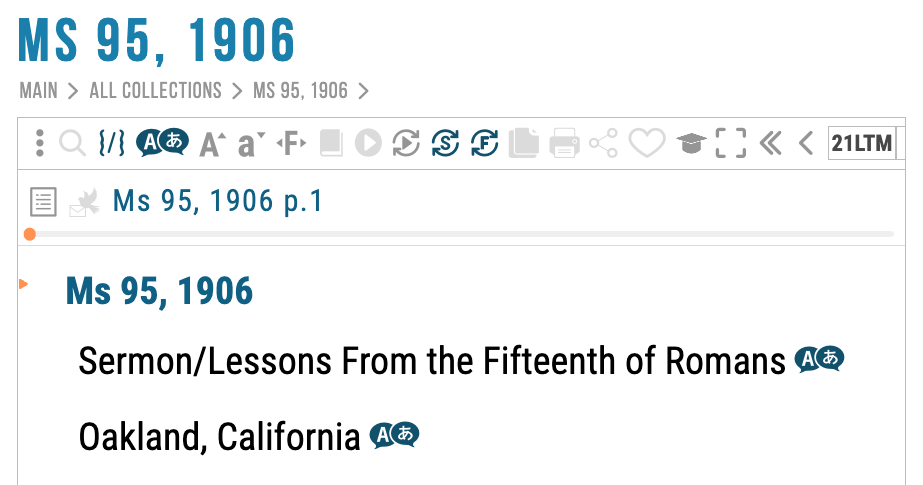
\includegraphics[width=1\linewidth]{images/sermons-and-talks.png}
    \label{fig:enter-label}
\end{figure}


\begin{figure}
    \centering
    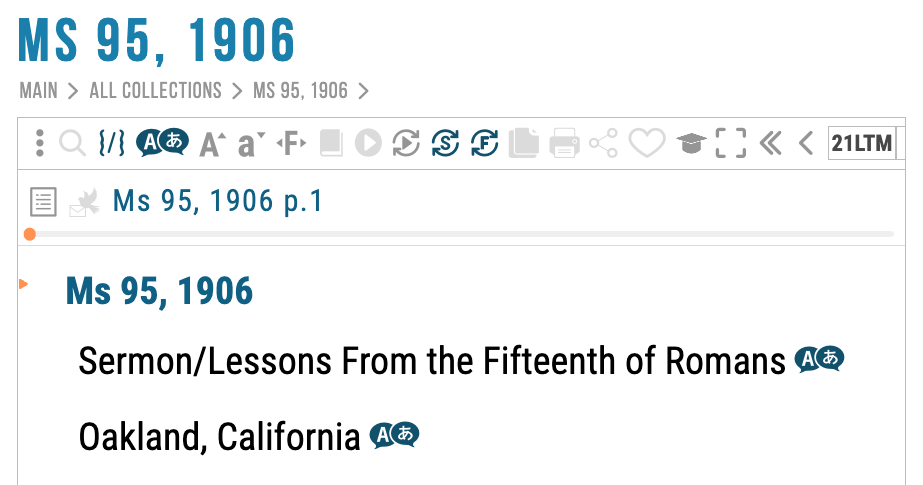
\includegraphics[width=1\linewidth]{images/sermons-and-talks.png}
    \label{fig:enter-label}
\end{figure}


For us, personally, these quotations are unauthenticated and, especially, invalid compared to Ellen White’s authenticated works. But if someone insists on weighing her unconfirmed reports and published writings equally, we will not stand in their way but even further push the conclusion of the Holy Spirit as a being. Let’s follow together.


بالنسبة لنا، شخصيًا، هذه الاقتباسات غير موثقة، وخاصة، غير صالحة مقارنة بأعمال إلين وايت الموثقة. ولكن إذا أصر أحد على وزن تقاريرها غير المؤكدة وكتاباتها المنشورة بالتساوي، فلن نقف في طريقهم بل سندفع أكثر نحو استنتاج الروح القدس ككائن. دعونا نتابع معًا.


Even compared with Ellen White’s authenticated works, such a Holy Spirit, a being, would not be one with God because Christ was \egwinline{\textbf{The only being who was one with God}}[Lt121-1897.7; 1897][https://egwwritings.org/read?panels=p7266.13]. This Holy Spirit, a being, could not \egwinline{\textbf{enter into all the counsels and purposes of God}}, because Christ was \egwinline{\textbf{the only being}}[PP 34.1; 1890][https://egwwritings.org/read?panels=p84.75] who could do that. This Being is not to be exalted because \egwinline{\textbf{The Father and the Son \underline{alone} are to be exalted}}[YI, July 7, 1898 par.2.; 1898][https://egwwritings.org/read?panels=p469.2964]. The Holy Spirit, as a being, would not fit in the order of heaven as the third being because Satan was \egwinline{\textbf{next to Christ the most exalted \underline{being}} in the heavenly courts}[RH August 9, 1898, par. 7; 1898][https://egwwritings.org/read?panels=p821.17145]. This Holy Spirit, a being, was not invested in the cost of salvation; neither was he in the covenant with Father and Son to save the world, nor dishonored by man’s transgression.


حتى بالمقارنة مع أعمال إلين وايت الموثقة، فإن مثل هذا الروح القدس، ككائن، لن يكون واحدًا مع الله لأن المسيح كان \egwinline{\textbf{الكائن الوحيد الذي كان واحدًا مع الله}}[Lt121-1897.7; 1897][https://egwwritings.org/read?panels=p7266.13]. هذا الروح القدس، ككائن، لا يمكنه \egwinline{\textbf{الدخول في جميع مشورات وأغراض الله}}، لأن المسيح كان \egwinline{\textbf{الكائن الوحيد}}[PP 34.1; 1890][https://egwwritings.org/read?panels=p84.75] الذي يمكنه فعل ذلك. هذا الكائن ليس ليتم تمجيده لأن \egwinline{\textbf{الآب والابن \underline{وحدهما} يجب أن يُمجَّدا}}[YI, July 7, 1898 par.2.; 1898][https://egwwritings.org/read?panels=p469.2964]. الروح القدس، ككائن، لن يتناسب مع نظام السماء كالكائن الثالث لأن الشيطان كان \egwinline{\textbf{التالي للمسيح أكثر \underline{كائن} ممجد}} في المحاكم السماوية}[RH August 9, 1898, par. 7; 1898][https://egwwritings.org/read?panels=p821.17145]. هذا الروح القدس، ككائن، لم يكن مستثمرًا في تكلفة الخلاص؛ ولم يكن في العهد مع الآب والابن لخلاص العالم، ولم يُهان بتعدي الإنسان.


\egwinline{The great gift of salvation has been placed within our reach at an \textbf{infinite cost to the Father and the Son}.}[RH November 21, 1912, par. 2; 1912][https://egwwritings.org/read?panels=p821.33329]


\egwinline{لقد وُضعت هبة الخلاص العظيمة في متناولنا \textbf{بتكلفة لا نهائية للآب والابن}.}[RH November 21, 1912, par. 2; 1912][https://egwwritings.org/read?panels=p821.33329]


\egwinline{In the plan to save a lost world, the counsel was between them \textbf{\underline{both}}; \textbf{the covenant of peace was between the Father and the Son}.}[ST December 23, 1897, par. 2; 1897][https://egwwritings.org/read?panels=p820.14803]


\egwinline{في خطة إنقاذ عالم ضائع، كان المشورة بينهما \textbf{\underline{كليهما}}؛ \textbf{كان عهد السلام بين الآب والابن}.}[ST December 23, 1897, par. 2; 1897][https://egwwritings.org/read?panels=p820.14803]


\egwinline{But in the transgression of man \textbf{\underline{both} the Father and the Son were dishonored}.}[ST December 12, 1895, par. 7; 1895][https://egwwritings.org/read?panels=p820.13243]


\egwinline{ولكن في تعدي الإنسان \textbf{\underline{كلاهما} الآب والابن أُهينا}.}[ST December 12, 1895, par. 7; 1895][https://egwwritings.org/read?panels=p820.13243]


Such a Holy Spirit, a being, does not fit into harmony with the authenticated reports of Ellen White, nor with the Scriptures. The Holy Spirit is called ‘\textit{spirit}’, so it is a spirit, exclusively.


مثل هذا الروح القدس، ككائن، لا يتناسق مع التقارير الموثقة لإلين وايت، ولا مع الكتب المقدسة. يُدعى الروح القدس ‘\textit{روح}’، لذا فهو روح، حصريًا.


Many of Sister White’s quotations are sourced from sermons or talks that were published after her death. In what follows, we will present a few that are most often discussed in an effort to prove that Sister White was a trinitarian. We invite everyone to weigh these quotations with her authenticated and published work, those during her lifetime.


العديد من اقتباسات الأخت وايت مصدرها عظات أو محادثات نُشرت بعد وفاتها. فيما يلي، سنقدم بعضًا من أكثر الاقتباسات التي تُناقش غالبًا في محاولة لإثبات أن الأخت وايت كانت تؤمن بالثالوث. ندعو الجميع لوزن هذه الاقتباسات مع أعمالها الموثقة والمنشورة، تلك التي نُشرت خلال حياتها.


“\textit{And then the golden harps are touched, and the music flows all through the heavenly host, and they fall down and worship the Father and the Son and the Holy Spirit}.”\footnote{\href{https://egwwritings.org/?ref=en_Ms139-1906.32&para=9579.38}{EGW; Ms139-1906.32; 1906}} [Sermon/Thoughts on Matthew 4. Oakland, California July 24, 1906; Previously unpublished.]


“\textit{وعندها تُعزف القيثارات الذهبية، وتتدفق الموسيقى عبر جميع الجموع السماوية، ويسقطون ويعبدون الآب والابن والروح القدس}.”\footnote{\href{https://egwwritings.org/?ref=en_Ms139-1906.32&para=9579.38}{EGW; Ms139-1906.32; 1906}} [عظة/أفكار حول متى 4. أوكلاند، كاليفورنيا 24 يوليو 1906؛ لم تُنشر سابقًا.]


“\textit{We need to realize that the Holy Spirit, who is as much a person as God is a person, is walking through these grounds.}”\footnote{\href{https://egwwritings.org/?ref=en_Ms66-1899.11&para=6622.19}{EGW; Ms66-1899.11: 1899}} [Talk/Extracts From Talks Given by Mrs. E. G. White at the Opening of College Hall, Avondale, and in the Avondale Church]


“\textit{نحتاج أن ندرك أن الروح القدس، الذي هو شخص بقدر ما الله هو شخص، يمشي عبر هذه الأراضي.}”\footnote{\href{https://egwwritings.org/?ref=en_Ms66-1899.11&para=6622.19}{EGW; Ms66-1899.11: 1899}} [حديث/مقتطفات من أحاديث قدمتها السيدة إ. ج. وايت في افتتاح قاعة الكلية، أفونديل، وفي كنيسة أفونديل]
